\chapter{Indledning}
\section{Krav til produktet}
Dette projekt tager udgangspunkt i projektoplægget for 3. Semester projektet, præsenteret af \textit{Ingeniørhøjskolen, Aarhus Universitet}. Til dette projekt er der ikke stillet krav til typen af produkt der skal udvikles, dog er der sat krav til hvad produket skal indeholde. Disse krav er som følge:

\begin{itemize}
	\item{Systemet \textit{skal} via sensorer/aktuatorer interagere med omverdenen}
	\item{Systemet \textit{skal} have en brugergrænseflade}
	\item{Systemet \textit{skal} indeholde faglige elementer fra semesterets andre fag}
	\item{Systemet \textit{skal} anvende en indlejret Linux platform og en PSoC platform}
\end{itemize}

På baggrund af disse krav er der udarbejdet et system, der beskrives i afsnit \ref{afsnit:systembeskrivelse}.

Til dette projekt bliver systemet opbygget som en prototype. Grundet dette er der i afsnit \ref{afsnit:analyse} beskrevet nogle grundlæggende hardwarekomponenter til realisering af denne prototype.

\section{Systembeskrivelse}
\label{afsnit:systembeskrivelse}
Ønsket med dette projekt er at udvikle en mekanisk enhed der kan styres med en håndholdt controller. Med dette udgangspunkt blev forskellige muligheder undersøgt som inspirationskilde, hvor valget herefter faldt på en kanon til affyring af slik. Ideen med en kanon der affyrer slik er ikke original, som det kan ses ud fra projektet \textit{"The Candy Cannon"} som er fundet på YouTube: \textbf{https://www.youtube.com/watch?v=VgZhQJQnnqA}. Til forskel fra \textit{The Candy Cannon} og lignende projekter som affyrer projektiler uden et egentlig formål, vil der i dette projekt blive udviklet en kanon til brug i et spil. Kanonen affyres og styres af spillerne via en controller. Altså skal projektet ende med en kanon som indgår i et to personersspil, f.eks. til brug ved fester og andre sociale begivenheder.

I dette projektet skal der altså udvikles en slikkanon til spillet \textit{Goofy Candygun 3000}. Denne slikkanon skal kunne skyde med slik. Dette kunne for eksempel være M\&M’s eller Skittle’s.

Goofy Candygun 3000 er et spil til to personer, hvilket gør det velegnet i sociale sammenhænge. Spillet går ud på at opnå flest point ved at ramme et mål. Hver spiller får et bestemt antal skud. Efter skuddene er opbrugt, er vinderen spilleren med flest point.

Et typisk brugerscenarie er, at spillerne bestemmer antallet af skud for runden. Når dette er gjort, er spillet igang. Herefter går Wii-nunchucken på skift mellem spillerne for hvert skud. Dette fortsættes indtil skuddene er opbrugt. Vinderen er spilleren med flest point. Spillets statistikker vises løbende på brugergrænsefladen. 

Det endelige produkt omfatter:
\begin{itemize}
	\item{En brugergrænseflade, hvor spilstatistikker fremvises til deltagerne. Dette er blandt andet:}
	\subitem{Pointvisning}
	\subitem{Kanonens vinkel}
	\subitem{Antal resterende skud}
	\item{En motor, der drejer kanonen om forskellige akser}
	\subitem{Dette styres med en Wii-nunchuck}
	\item{Et mål, der kan registrere spillernes skud}
\end{itemize}

Med baggrund i krav stillet af organisationen IHA, bliver produktet udviklet med følgende funktioner:

\begin{itemize}
	\item DevKit 8000 som den indlejrede linux-platform til spillets grafiske brugergrænseflade.
	\item Motorer til styring af kanonen.
	\item Sensorer.
	\item PSoC 4, anvendt til styring af motorer og kommunikation med sensorer.
\end{itemize}

\newpage
\section{Rigt Billede}

På figur \ref{ref:RigtBillede} ses et rigt billede af det ønskede produkt. Billedet beskriver brugerscenariet.

\begin{figure}[H]
	\centering
	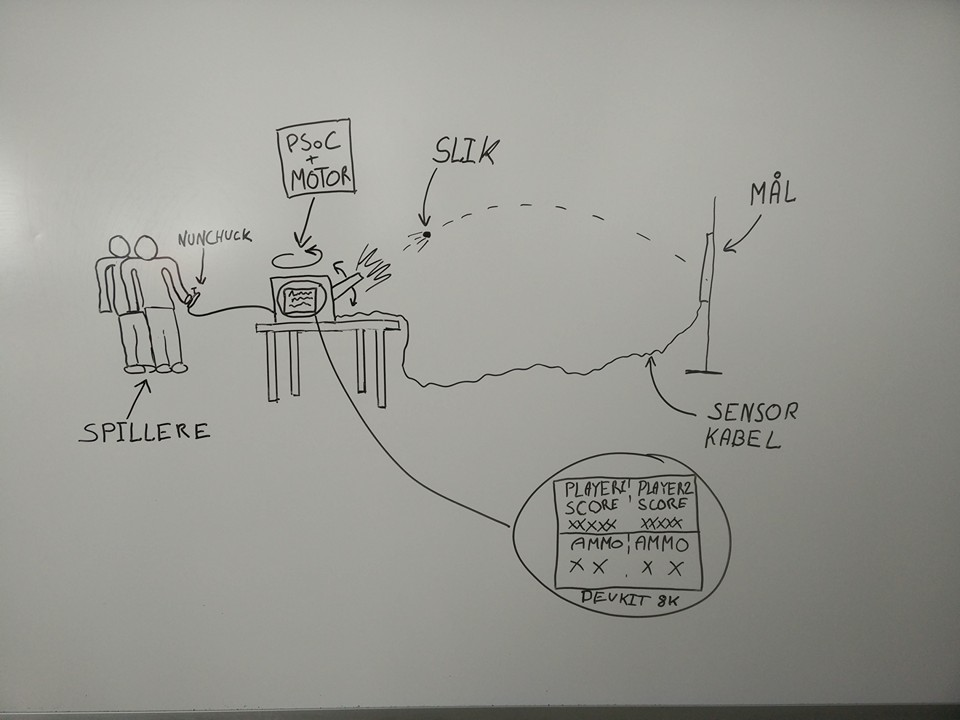
\includegraphics[width=\textwidth]{Projektformulering/images/rigtBillede}
	\caption{Rigt Billede af det endelige produkt}
	\label{ref:RigtBillede}
\end{figure}

\newpage
\section{Ansvarsområder}
I løbet af projektet vil projektgruppen blive opdelt i to hovedgrupper - 'hardware' og 'software'. Softwaregruppen vil desuden stå for grænsefladeprogrammering mellem software og hardware. Disse grupper vil have til ansvar at designe og implementere hhv. hardware og software til projektet. Hardwaregruppen vil bestå af de personer, der læser til elektroingeniør (Mikkel Nielsen og Pernille Kjeldgaard). Softwaregruppen vil bestå af de personer, der læser til IKT-ingeniør (Kasper Rieder, Michael Kloock, Tenna Rasmussen, Mia Konstmann og Daniel Jensen).

På tabel \ref{tabel:ansvarsområder} ses opdelingen af ansvarsområder mellem projektgruppens medlemmer. Her bruges bogstavet \textit{P} til at angive \textit{primært} ansvar, hvor bogstavet \textit{S} angiver \textit{sekundært} ansvar.

\begin{table}[H]
	\centering
	\begin{tabular}{llllllll}
		\hline
		\multicolumn{1}{|l|}{Ansvarsområder}     & \rot{Daniel Jensen }& \rot{Mia Konstmann } & \rot{Mikkel Nielsen } & \rot{Kasper Rieder } & \rot{Michael Kloock } & \rot{Tenna Rasmussen } & \rot{Pernille Kjeldgaard } \\ \hline
		\rowcolor[HTML]{CBCEFB} 
		I2C Kommunikationsprotokol PSoC Software & P                        & S                        &                         & P                       &                          &                         &                          \\
		Nunchuck PSoC Software                   & S                        & P                        &                         & S                       &                          &                         &                          \\
		\rowcolor[HTML]{CBCEFB} 
		SPI Kommunikationsprotokol PSoC Software & P                        & S                        &                         & P                       &                          &                         &                          \\
		SPI Driver Devkit Software               &                          & S                        &                         & S                       &                          & P                       &                          \\
		\rowcolor[HTML]{CBCEFB} 
		Brugergrænseflade Devkit Software        &                          &                          &                         &                         & P                        &                         &                          \\
		Motorstyring PSoC Software               &                          & P                        & P                       & S                       &                          &                         &                          \\
		\rowcolor[HTML]{CBCEFB} 
		Use Case 2 Implementering                & P                        & S                        &                         & P                       &                          &                         &                          \\
		&                          &                          &                         &                         &                          &                         &                          \\
		\rowcolor[HTML]{CBCEFB} 
		H-bro                                    &                          &                          &                         &                         &                          &                         &                          \\
		Affyringsmekanisme                       &                          &                          &                         &                         &                          &                         &                         
	\end{tabular}
		\caption{Ansvarsområder tabel}
		\label{ansvarsområder}
\end{table}